\section{Reinforcement Learning}
\begin{figure}[!h]
    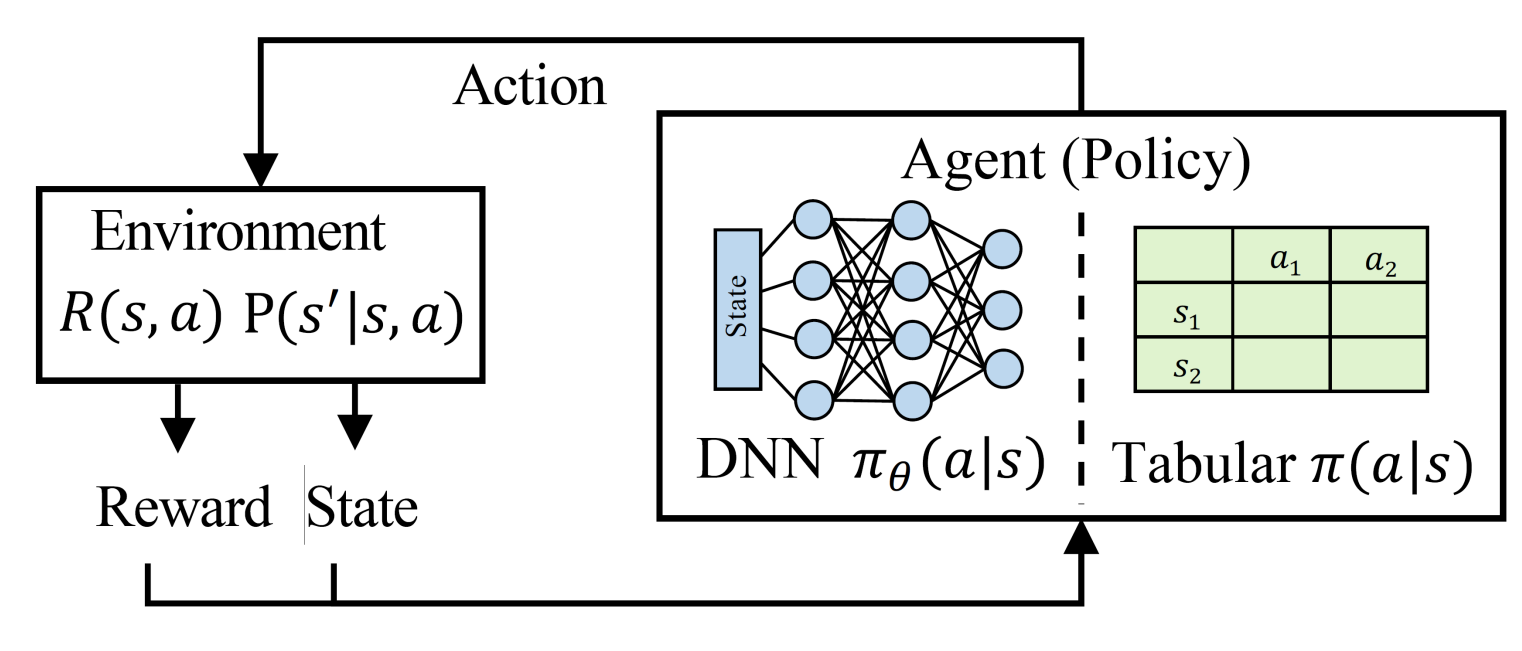
\includegraphics[width = \columnwidth]{figures/13/AgentEnvironment.png}    
\end{figure}
The agent and environment interact at each of a sequence of discrete time steps,\(t = 0,1,2,\dots\).
At each time step \(t\), the agent receives some representation of the environment's states,\(s_i \in S\), where \(S\) is the set possible states.
On that basis, the agent selects an action, \(a\in A(s_t)\), where \(A(s_t)\) is the set of actions available in state \(s_t\).
One time step later, in part as a consequence of its action, the agent receives a numerical reward,\(R_{t+1}\in \mathbb{R}\), and finds itself in a new state, \(s_{t+1}\).
\subsubsection{Policy \(\pi\)}
A policy \(\pi\) is a distribution over actions \(a\) given state \(s\),i.e. it is the probability that the agent takes action \(a_t \in A\) in state \(s \in S\)
\[
\pi(a|s) = Pr\left[a_t = a|s_t = s\right]
\]
\subsubsection{Types of RL environments}
\begin{itemize}
    \item Deterministic environment
    \item Stochastic environment
    \item Fully observeable environment
    \item Partially observeable environment
    \item Discrete environment
    \item Continuous environment
    \item Episodic and non-episodic environment
    \item Single and multi-agent environment
\end{itemize}
\subsubsection{Agent Categories}
\begin{itemize}
    \item Value Based: No policy, Value function
    \item Policy Based: Policy, No value function
    \item Actor Critic: Policy(for the actor), Value function (for the critic)
    \item Model Free: Policy and/or Value function, no (explicit) Model of the Environment, no explicit dynamics Model
    \item Model Based: Optionally Policy and/or Value function, (explicit) Model of the Environment, explicit dynamics Model
\end{itemize}
\subsubsection{Markov Process}
A Markov Process (or Markov Chain) is a tuple (S,P), where:
\begin{itemize}
    \item \(S\) is a (finite) set of states
    \item \(P\) is a state transition probability matrix(Markov table): \(P_{ss'} = Pr(s_{t+1}|s_t)\)
\end{itemize}
The core concept is that the future only depends in the present and not on the past.
\subsubsection{Markov Reward Process (MRP)}
A Markov Reward Process is a tuple \((S,P,\mathcal{R},\gamma)\):
\begin{itemize}
    \item \(S\) is a (finite) set of states
    \item \(P\) is a state transition probability matrix:\(P = P_{ss'} = Pr(s_{t+1}|s_t)\)
    \item \(\mathcal{R}\) is a reward function (expectation value of the next reward): \(\mathcal{R}_s = \mathbb{E}\left[R_{t+1}|s_t\right]\)
    \item \(\gamma\) is a discount factor: \(\gamma \in \left[0,1\right]\)
\end{itemize}
\subsection{Markov decision process (MDP = MRP + A)}
A Markov Decision Process is a tuple \((S,A,P,\mathcal{R},\gamma)\)
\begin{itemize}
    \item \(S\) is a (finite) set of states
    \item \(A\) is a (finite) set of actions
    \item \(P\) is a state transition probability matrix:\(P = P_{ss'} = Pr(s_{t+1}|s_t)\)
    \item \(\mathcal{R}\) is a reward function (expectation value of the next reward): \(\mathcal{R}_s = \mathbb{E}\left[R_{t+1}|s_t\right]\)
    \item \(\gamma\) is a discount factor: \(\gamma \in \left[0,1\right]\)
\end{itemize}

\subsubsection{Return \(G_t\)}
The Return \(G_t\) is the total discounted reward from time-step \(t\) on.
\[
G_t = R_{t+1} + \gamma R_{t+2} + \dots = \sum_{k = 0}^{\infty} \gamma^k R_{t+k+1}
\]
\begin{itemize}
    \item \(\gamma\) close to 0 leads to myopic evaluation
    \item \(\gamma\) close to 1 leads to far-sighted evaluation
\end{itemize}
Recursion formula (basis for the Bellman equation):
\[
G_t = R_{t+1} + \gamma G_{t+1}
\]
\subsubsection{Value Function \(V(s)\) and Bellman Equation for MRP}
The state-value-function \(V(s)\) of an MRP is the expected cumulated return starting from state \(s\);
\[
V(s) = \mathbb{E}\left[G_t|s_t = s\right]
\]
The state-value-function can be decomposed in two parts.
This leads to the Bellman Equation for MRPs
\[
\mathcal{R}_s = \mathbb{E}_\pi\left[R_{t+1}|s_t\right]
\]